Jak już wspomniano, w Polsce centralnym organem odpowiedzialnym
za przyznawanie patentów jest \acf{UPRP}. Oprócz ochroną patentową
oraz publikowaniem informacji o patentach, urząd prowadzi
bazę danych patentów, która jest dostępna publicznie przy użyciu \ac{API}.
Pozwala to na automatyczne pobieranie danych przy pomocy skryptów.

\section{\ac{UPRP}}\label{sec:UPRP}

Identyfikacja patentów w tym systemie to przyporządkowanie
każdego patentu do 6-cyfrowego numeru, który jest unikalny dla
każdego zgłoszenia. Pobieranie danych dotyczących wszystkich patentów 
można więc przeprowadzić wysyłając zapytanie do interfejsu o każdy
patent po kolei. W odpowiedzi otrzymuje się dane w formacie \ac{XML}.

\bigskip
\begin{figure}
\centering
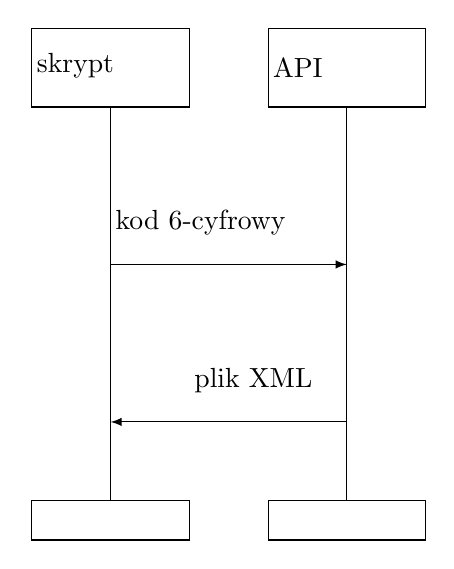
\begin{tikzpicture}
	\draw[draw=black, thin, solid] (-3.00,3.00) rectangle (-1.00,2.00);
	\draw[draw=black, thin, solid] (0.00,3.00) rectangle (2.00,2.00);
	\node[black, anchor=south west] at (-3.06,2.25) {skrypt};
	\node[black, anchor=south west] at (-0.06,2.25) {\ac{API}};
	\draw[draw=black, thin, solid] (-2.00,2.00) -- (-2.00,-3.00);
	\draw[draw=black, thin, solid] (1.00,2.00) -- (1.00,-3.00);
	\node[black, anchor=south west] at (-2.06,0.25) {kod 6-cyfrowy};
	\draw[draw=black, -latex, thin, solid] (-2.00,0.00) -- (1.00,0.00);
	\node[black, anchor=south west] at (-1.06,-1.75) {plik XML};
	\draw[draw=black, -latex, thin, solid] (1.00,-2.00) -- (-2.00,-2.00);
	\draw[draw=black, thin, solid] (-3.00,-3.00) rectangle (-1.00,-3.50);
	\draw[draw=black, thin, solid] (0.00,-3.00) rectangle (2.00,-3.50);
\end{tikzpicture}
\caption{Schemat pobierania danych z \ac{API} \ac{UPRP}}
\end{figure}

\subsection{Dane w formie surowej}
\label{sec:profilowanie-UPRP}

Wstępna struktura to formacja zagnieżdzonych obiektów z parametrami 
oraz list obiektów innego typu. Zagnieżdżenie oznacza, że obiekt znajduje się
w innym obiekcie, a parametr to wartość skalarna przyporządkowana danej obserwacji.
Dodatkowo każdy dokument traktujemy także jako obiekt.
Ze względów praktycznych dane wymagają wstępnej obróbki.
Pożądana struktura to listy obiektów ustalonego typu, z parametrami, 
bez żadnych zagnieżdżeń.

\bigskip

\begin{figure}[H]
\begin{tikzpicture}
	\draw[draw=black, thin, solid] (-6.00,5.00) rectangle (8.00,-6.00);
	\draw[draw=black, thin, solid] (3.00,-2.00) rectangle (0.00,-5.00);
	\draw[draw=black, thin, solid] (-1.00,-2.00) rectangle (-4.00,-5.00);
	\draw[draw=black, thin, solid] (-4.00,3.00) rectangle (-1.00,0.00);
	\draw[draw=black, thin, solid] (0.00,3.00) rectangle (3.00,0.00);
	\draw[draw=black, thin, solid] (-5.00,4.00) rectangle (7.00,-1.00);
	\node[black, anchor=south west] at (-6.06,5.25) {$A_1$};
	\node[black, anchor=south west] at (-0.06,3.25) {$C_2$};
	\node[black, anchor=south west] at (-4.06,3.25) {$C_1$};
	\node[black, anchor=south west] at (-4.06,-1.75) {$B_2$};
	\node[black, anchor=south west] at (-5.06,4.25) {$B_1$};
	\node[black, anchor=south west] at (-0.06,-1.75) {$G$};
	\node[black, anchor=south west] at (-3.56,2.25) {$c_1: x_1$};
	\node[black, anchor=south west] at (-3.56,1.25) {$c_b: x_2$};
	\node[black, anchor=south west] at (-3.56,0.25) {$c_r: x_3$};
	\node[black, anchor=south west] at (0.44,2.25) {$c_1: x_4$};
	\node[black, anchor=south west] at (0.44,0.25) {$c_3: x_5$};
	\node[black, anchor=south west] at (4.44,2.25) {$b_1: x_6$};
	\node[black, anchor=south west] at (-3.56,-2.75) {$b_1: x_7$};
	\node[black, anchor=south west] at (-3.56,-3.75) {$b_2: x_8$};
	\node[black, anchor=south west] at (-3.56,-4.75) {$b_3: x_9$};
	\node[black, anchor=south west] at (0.44,-2.75) {$g_1: x_{10}$};
	\node[black, anchor=south west] at (0.44,-3.75) {$g_2: x_{11}$};
	\node[black, anchor=south west] at (4.44,-2.75) {$a_1: x_{12}$};
	\node[black, anchor=south west] at (4.44,-3.75) {$a_2: x_{13}$};
\end{tikzpicture}
    \centering
    \caption{Przykładowy schemat danych zagnieżdżonych}
    \label{fig:przykład-danych}
\end{figure}

W powyższym przykładzie zaprezentowany jest dokument $A_1$ o nazwie $A$.
Dla dokumentów jest przyjęte, że jest to relatywna ścieżka lokacji,
w której się znajdują na urządzeniu.

Obiekt $A_1$ zawiera 2 parametry i 3 obiekty:

\begin{itemize}
  \item parametry mają klucze $a_1$ oraz $a_2$ z wartościami, odpowiednio, 
        $x_{12}$ oraz $x_{13}$;
  \item 2 obiekty $B_1$ oraz $B_2$ o nazwie $B$;
  \item obiekt typu $G_1$ nazywa się $G$.
\end{itemize}

\Needspace{7\baselineskip}
Ścieżki to ciągi nazw obiektów i parametrów, które trzeba przejść, 
aby dotrzeć do wartości. Dla wyżej wymienionych właśności będą to odpowiednio:

\begin{itemize}
  \item $a_1\colon\quad(A, a_1)$
  \item $a_2\colon\quad(A, a_2)$
  \item $B_1\colon\quad(A, B)$
  \item $B_2\colon\quad(A, B)$
  \item $G_1\colon\quad(A, G)$
\end{itemize}

Dla wartości $c_3$ w obiekcie $C$ ścieżką będzie $c'_3=(A, B, C, c_3)$.

Z faktu, że istnieją 2 obiekty jednego typu $B$ wnosimy, że jest 
to lista obiektów i na tej podstawie definiujemy typ $T_B$.
Wszystkie obiekty o identycznej ścieżce $(A, B)$. Schemat
przedstawia sytuację, w której mimo takiej samej ścieżki, co za tym
idzie, identycznego typu jest istotna różnica w strukturze obu obiektów.
W takiej sytuacji przyjmowane jest, że to większy zbiór kluczy definiuje
parametry obiektu, a różnice są przyjmowane jako braki w poszczególnych
obiektach: $B_1 = \{ b'_1 = x_7; b'_2 = x_8; b'_3 = x_9 \}$,
$B_2 = \{ b'_1 = x_6; b'_2 = \emptyset; b'_3 = \emptyset \}$.

Jak widać w strukturach $B_1$ oraz $B_2$ nie wymieniamy faktu,
że mogą zawierać obiekty o nazwie $C$. To $C_1$ oraz $C_2$ są
powiązane do obiektów nadrzędnych poprzez nadanie im nowych
parametrów, które zawierają unikalny klucz obiektu nadrzędnego.

Każdy obiekt ma generowany własny unikalny klucz.

Jeszcze jedną wartą uwagi sytuacją jest to jak traktowany jest 
obiekt $G_1$. Jak widać jest on jedyny w obiekcie $A_1$, stąd
nie będzie traktowany jako obiekt w danych wyjściowych. Jego
parametry będą parametrami obiektu $A_1$ co da obraz obiektu $A_1$
jako $\{a'_1 = x_{12}, a'_2 = x_{13}, g'_1 = x_{10}, g'_2 = x_{11} \}$.

W sytacji, w której inny dokument $A$ miałby przynajmniej dwa obiekty
o nazwie $G$ sytuacja była by analogiczna do sytuacji obiektów $C_1; C_2$



\subsubsection{Zasada profilowania danych}

Głównym problemem jest fakt, że dane są rozległe oraz różnią się 
w schemacie w zależności od czasu dodania oraz wolumenu i jakości informacji
jakie zostały wprowadzone w każdym przypadku.

Aby wyróżnić typy obiektów przyjmujemy, że każdy parametr ma dokładnie 1 obiekt,
a każdy obiekt ma dokładnie 1 parametr o danej ścieżce. Ścieżka to ciąg nazw
obiektów jakie należy przejść, aby dotrzeć do wskazanego obiektu w zagnieżdżonej
strukturze. Jeśli w obiekcie istnieją 2 obiekty o identycznej ścieżce to przyjmujemy,
że znajdują się w liście obiektów tego samego typu. Właśnie tak wyróżniamy typ.
Jeśli taka sytuacja dzieje się tylko dla części dokumentów, to i tak 
przyjmujemy je jako elementy wyróżnionego typu, a nie parametry obiektu
aby zapewnić homogeniczność danych. Podobnie dzieje się w przypadku braków:
jeśli część obiektów tego samego typu ma pewien parametr, a część go nie ma
to przyjmujemy, że i tak ten parametr jest charakterystyczny dla tego typu.
Część obiektów po prostu nie ma tej informacji.

Implementacja polega na zastosowaniu 2 etapów: wyszukiwania powtarzających się
ścieżek i wyróżniania ich jako typy obiektów, oraz etap drugi: zbieranie danych
do tabel zgodnie z wyróżnionymi typami obiektów.

W trakcie tych procesów występują także inne działania, takie jak określanie
unikalnych numerów identyfikacyjnych każdego obiektu, wiązanie obiektów ze sobą
za pomocą umieszczania identyfikatorów obiektów nadrzędnych w tych podrzęndnych,
każda tabela zawiera numer dokumentu, z którego pochodzi, numeracja obiektów i
dokumentów jest generowana na bieżąco i nie ma związku z danymi po za tym, że
to na podstawie ich steuktury powstaje, nazwy tabel i parametrów to ścieżki
jakimi są podpisane.

\Needspace{30\baselineskip}
Po zastosowaniu procesu, dla wcześniej wymienionego przykładu 
\cref{fig:przykład-danych} należy oczekiwać następujących niżej danych, 
patrz: \cref{fig:przykład-danych-po-profilowaniu}.

\begin{uwaga}
W tym przypadku zakładamy, że obiekt $G$ nigdy nie 
występuje wielokrotnie w dokumencie. To jak zachowuje się obiekt
występujący wielokrotnie przedstawia $B$ oraz $C$.
\end{uwaga}

\begin{figure}[H]\centering
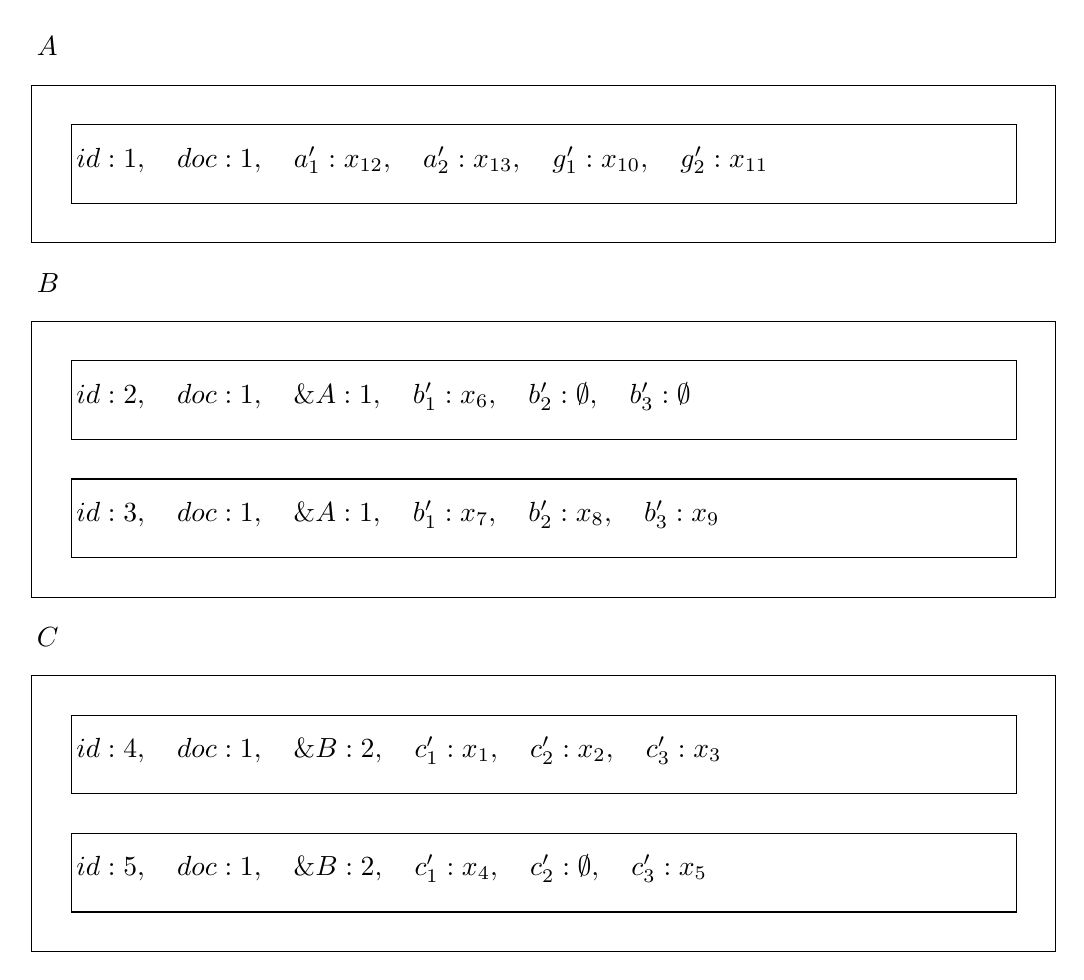
\begin{tikzpicture}
\node[black, anchor=south west] at (-4.56,0.75) {$A$};
\node[black, anchor=south west] at (-4.06,-0.75) {
\begin{math}
\text{id}: 1,\quad
\text{doc}: 1,\quad
a'_1: x_{12},\quad
a'_2: x_{13},\quad
g'_1: x_{10},\quad
g'_2: x_{11}
\end{math}
};
\draw[draw=black, thin, solid] (-4.00,-1.00) rectangle (8.00,0.00);
\draw[draw=black, thin, solid] (-4.50,0.50) rectangle (8.50,-1.50);
\draw[draw=black, thin, solid] (-4.50,-2.50) rectangle (8.50,-6.00);
\draw[draw=black, thin, solid] (-4.00,-3.00) rectangle (8.00,-4.00);
\draw[draw=black, thin, solid] (-4.00,-4.50) rectangle (8.00,-5.50);
\node[black, anchor=south west] at (-4.56,-2.25) {$B$};
\node[black, anchor=south west] at (-4.06,-3.75) {
\begin{math}
\text{id}: 2,\quad
\text{doc}: 1,\quad
\text\&{A}: 1,\quad
b'_1: x_{6},\quad
b'_2: \emptyset,\quad
b'_3: \emptyset
\end{math}
};
\node[black, anchor=south west] at (-4.06,-5.25) {
\begin{math}
\text{id}: 3,\quad
\text{doc}: 1,\quad
\text\&{A}: 1,\quad
b'_1: x_{7},\quad
b'_2: x_{8},\quad
b'_3: x_{9}
\end{math}
};
\draw[draw=black, thin, solid] (-4.50,-7.00) rectangle (8.50,-10.50);
\draw[draw=black, thin, solid] (-4.00,-7.50) rectangle (8.00,-8.50);
\draw[draw=black, thin, solid] (-4.00,-9.00) rectangle (8.00,-10.00);
\node[black, anchor=south west] at (-4.56,-6.75) {$C$};
\node[black, anchor=south west] at (-4.06,-8.25) {
\begin{math}
\text{id}: 4,\quad
\text{doc}: 1,\quad
\text\&{B}: 2,\quad
c'_1: x_{1},\quad
c'_2: x_{2},\quad
c'_3: x_{3}
\end{math}
};
\node[black, anchor=south west] at (-4.06,-9.75) {
\begin{math}
\text{id}: 5,\quad
\text{doc}: 1,\quad
\text\&{B}: 2,\quad
c'_1: x_{4},\quad
c'_2: \emptyset,\quad
c'_3: x_{5}
\end{math}
};
\end{tikzpicture}
\caption{Schemat danych zagnieżdżonych (patrz: \cref{fig:przykład-danych}) po profilowaniu}
\label{fig:przykład-danych-po-profilowaniu}
\end{figure}



\subsubsection{Tworzenie uproszczonych nazw tabel i kolumn}

Ostatecznie otrzymujemy kilka tabel, które są powiązane między sobą identyfikatorami.
Ich nazwy oraz nazwy parametrów to ścieżki w oryginalnej strukturze. Aby ułatwić
czytelność danych wymagany jest kolejny etap aliasowania. Polega on na przypisaniu
unikalnej nazwy. Nazwy powstają ze ścieżek jako ich podciagi. Generowanie opiera się
o stworznie grafu drzewa, w którym każdy wierzchołek to fragment ścieżki. Wierzchołki
zawierają informacje, które ścieżki używają fragmentów przypisanych do nich.
Nazwy powstają przez pobranie ostatniego wierzchołka; dalej jeśli taka nazwa
jest unikalna zostaje zapisana, jeśli nie dodawany jest kolejny wierzchołek, który
nie został wcześniej użyty, jeśli to niemożliwe dodawany jest jakikolwiek wierzchołek,
a później sytuacja się powtarza do osiągnięcia unikalności. W przypadku porażki dodawany
jest iteracyjnie numer, który i tak zapewnia unikalność. Oryginalne ścieżki
wraz z nazwami są zapisane jako słownik, aby nie tracić informacji. Natomiast
tabele i ich kolumny przyjmują nowe unikalne nazwy prostsze w obróce.

\needspace{20\baselineskip}
Dla przykładu \ref{fig:przykład-danych} należy oczekiwać następujących ścieżek:

\begin{itemize}
\item $(A) \to (A)$
\item $(A, B) \to (A, B)$
\item $(A, B, b_1) \to (A, b_1)$
\item $(A, B, b_2) \to (A, b_2)$
\item $(A, B, b_3) \to (A, b_3)$
\item $(A, B, C) \to (A, C)$
\item $(A, B, C, c_1) \to (A, c_1)$
\item $(A, B, C, c_2) \to (A, c_2)$
\item $(A, B, C, c_3) \to (A, c_3)$
\item $(A, G, g_1) \to (A, g_1)$
\item $(A, G, g_2) \to (A, g_2)$
\end{itemize}

\needspace{20\baselineskip}
Częstą sytuacją jest to, że nazwy parametrów są identyczne,
zakładając, że $b_1 = g_1$ otrzymalibyśmy dla nich następujące
ścieżki o zapewnionej unikalności:

\begin{itemize}
\item $(A) \to (A)$
\item $(A, B) \to (A, B)$
\item $(A, B, b_1) \to (A, b_1)$
\item $(A, B, b_2) \to (A, b_2)$
\item $(A, B, b_3) \to (A, b_3)$
\item $(A, B, C) \to (A, C)$
\item $(A, B, C, c_1) \to (A, c_1)$
\item $(A, B, C, c_2) \to (A, c_2)$
\item $(A, B, C, c_3) \to (A, c_3)$
\item $(A, G, g_1) \to (A, G, g_1)$ --- 
      dodatkowa wartość $G$ w ścieżce
\item $(A, G, g_2) \to (A, g_2)$
\end{itemize}


\newpage
\footnotesize
\input{ex-storage/input}
\normalsize
\newpage




\subsection{Przypisywanie ról dla danych}

Po wyciągnięciu danych dla każdego rodzaju wartości można 
przypisać rolę. W toku dalszej analizy, role są używane do
wyciągania danych o różnych formatach z wielu tabel jednocześnie
do homogenicznych struktur. Struktury składają się z wyciągnietych
wartości oraz ich mapowania do oryginalnych danych.
To podejście zapewnia względną jednorodność oczekiwanych danych
dzięki zastosowaniu powtarzalnej metody ich wyciągania;
mapowanie daje wgląd do wewnętrznych źródeł danych; dane oryginalne
po profilowaniu nigdy nie zmieniają formy.

\sidenote{czy potrzebne wyjaśn.?}